\chapter{Results of the ideal data validation}
\label{app:B}

In this appendix all the kinematic signals of the bicycle model that were checked in order to validate the ideal data, are presented. The lane change used for validation has as initial speed $22.22 \frac{m}{s}$ and uses a desired lateral distance of $3.47 \hspace{1mm}m$. First the different results of varying the time limit are shown and next come the results with regard to varying the amount of control points $N$.


\section{Time limit}

\begin{figure}[h!]
	\centering
	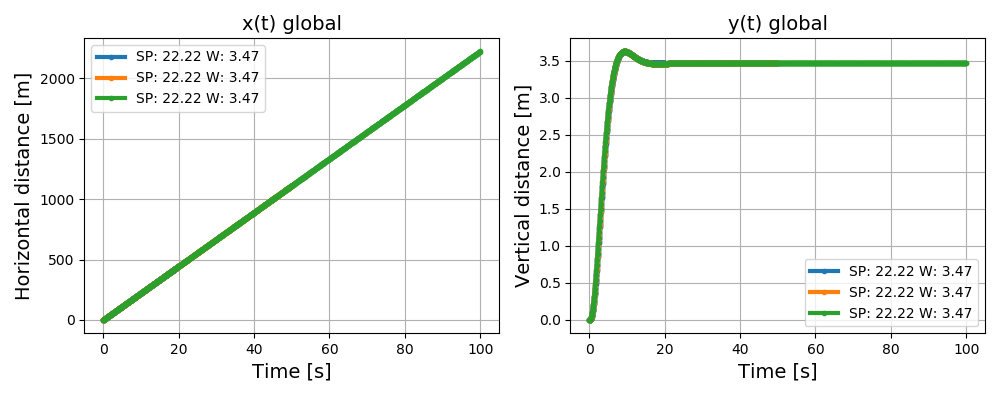
\includegraphics[width=1.0\textwidth]{1t.png}
	\label{fig:lat_acc_val}
\end{figure}


\begin{figure}[h!]
	\centering
	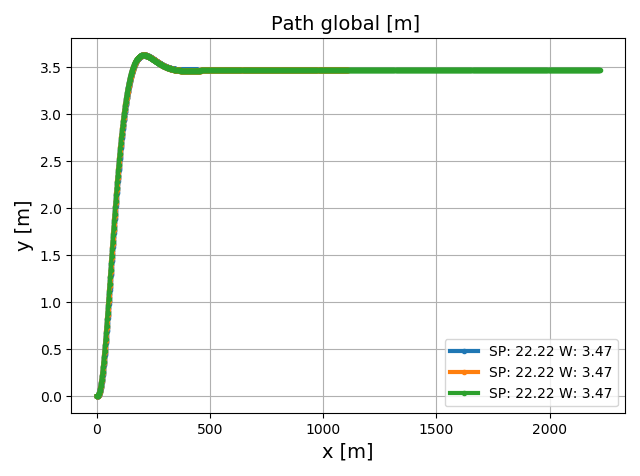
\includegraphics[width=0.8\textwidth]{2t.png}
	\label{fig:lat_acc_val}
\end{figure}

\begin{figure}[h!]
	\centering
	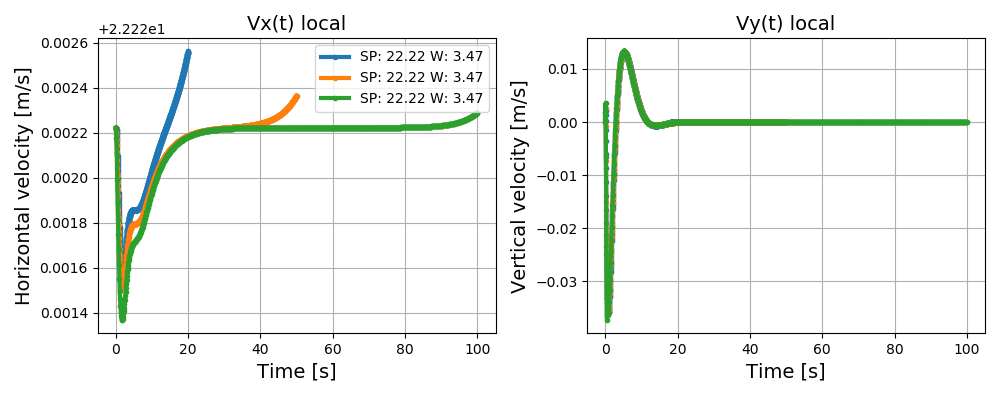
\includegraphics[width=1.0\textwidth]{3t.png}
	\label{fig:lat_acc_val}
\end{figure}


\begin{figure}[h!]
	\centering
	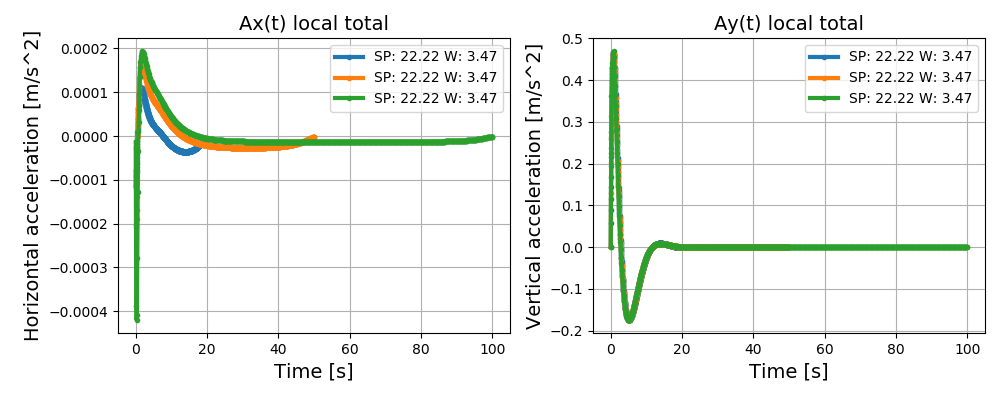
\includegraphics[width=1.0\textwidth]{4t.png}
	\label{fig:lat_acc_val}
\end{figure}


\begin{figure}[h!]
	\centering
	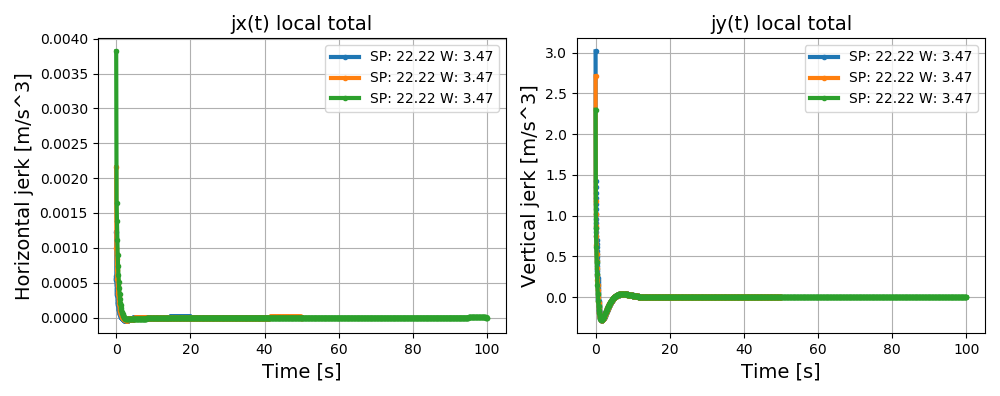
\includegraphics[width=1.0\textwidth]{5t.png}
	\label{fig:lat_acc_val}
\end{figure}


\begin{figure}[h!]
	\centering
	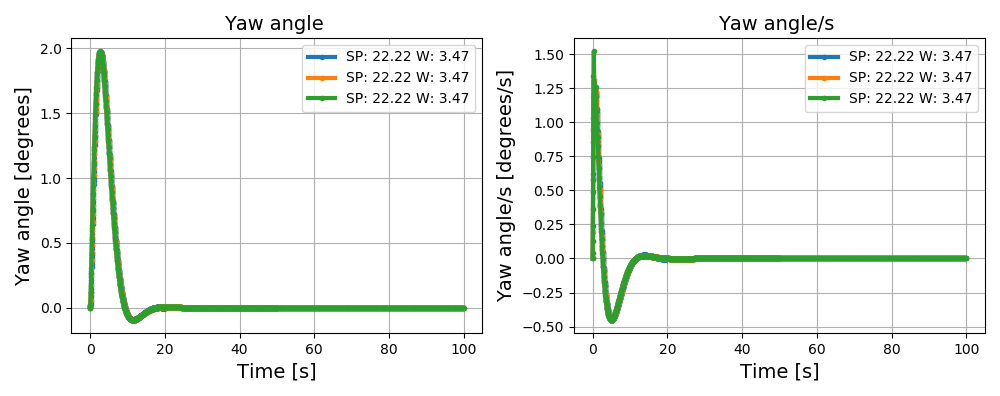
\includegraphics[width=1.0\textwidth]{6t.png}
	\label{fig:lat_acc_val}
\end{figure}


\begin{figure}[h!]
	\centering
	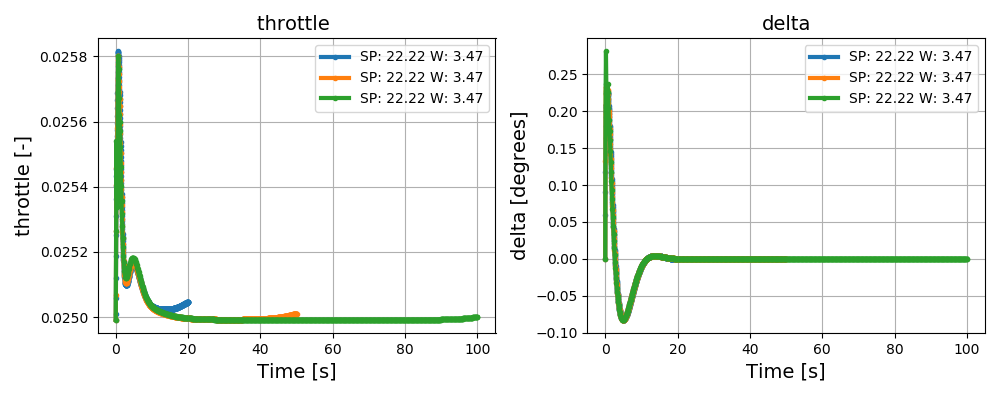
\includegraphics[width=1.0\textwidth]{7t.png}
	\label{fig:lat_acc_val}
\end{figure}


\begin{figure}[h!]
	\centering
	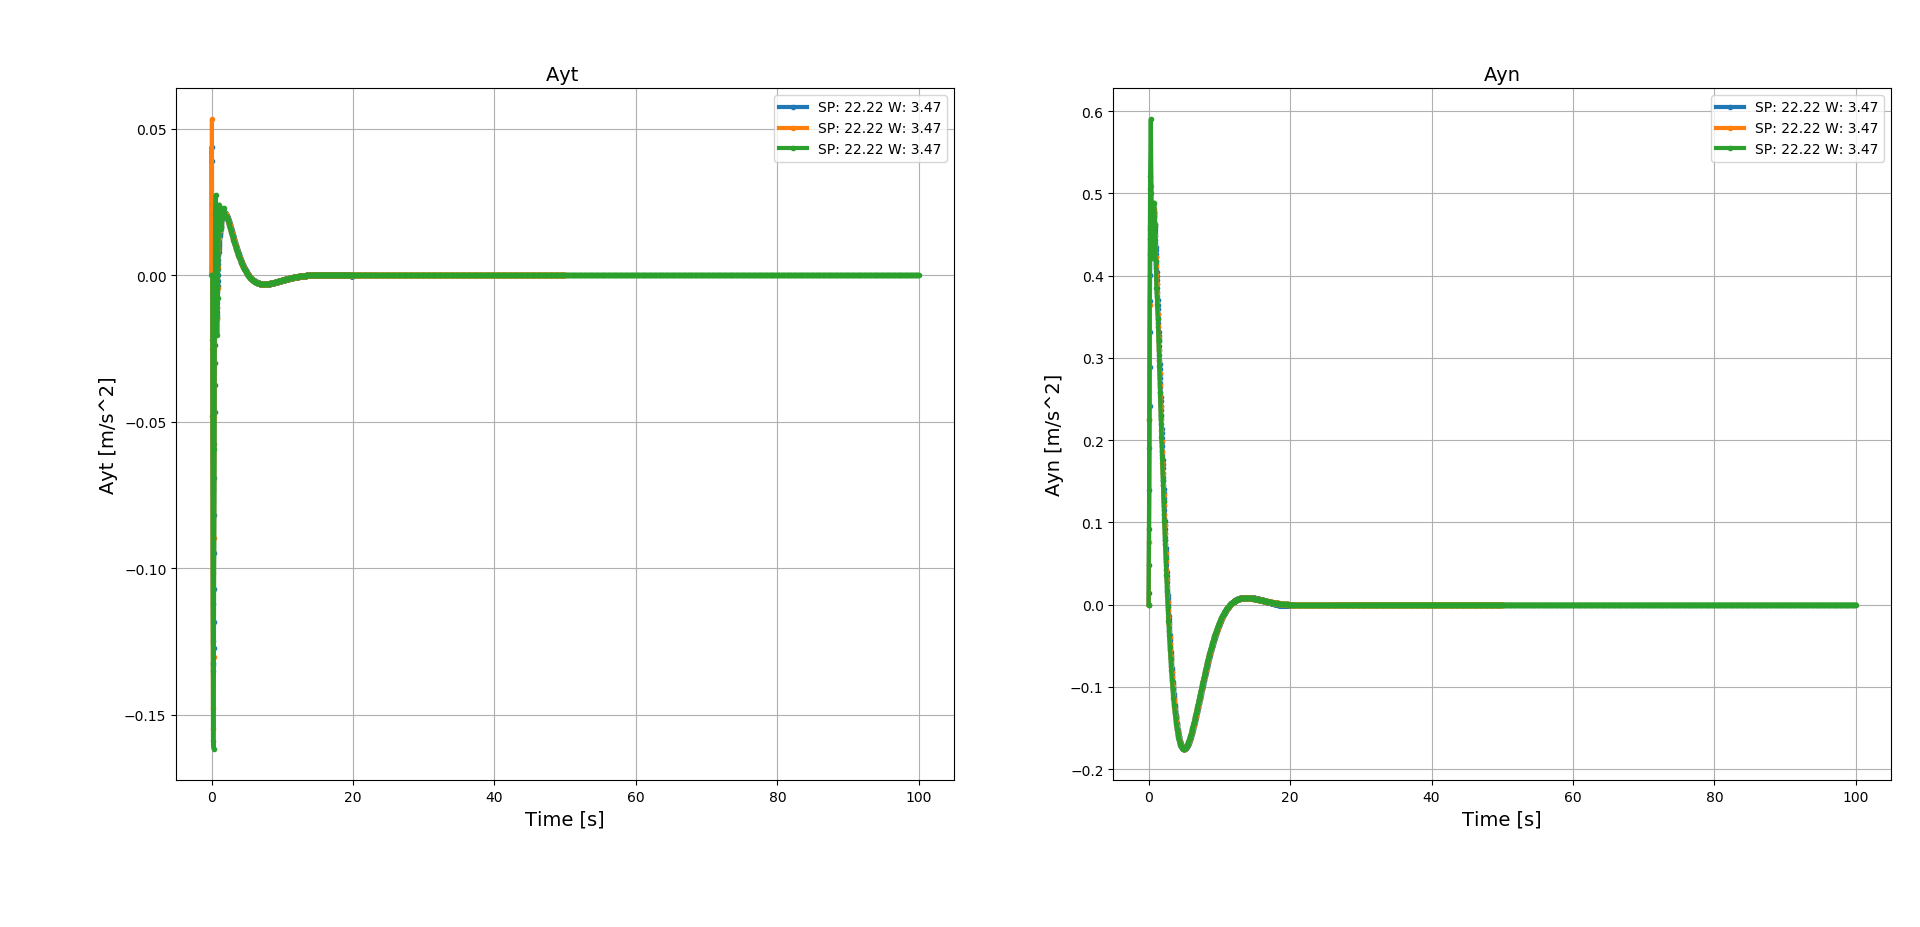
\includegraphics[width=1.1\textwidth]{8t.png}
	\label{fig:lat_acc_val}
\end{figure}


\begin{figure}[h!]
	\centering
	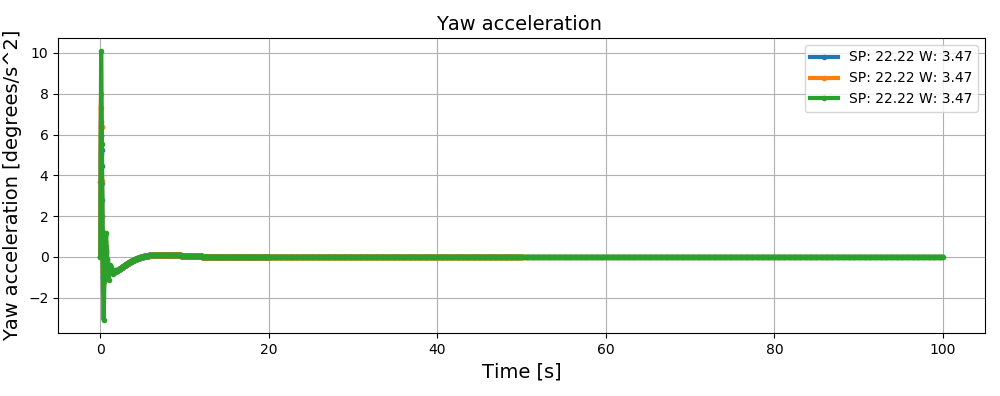
\includegraphics[width=1.0\textwidth]{9t.png}
	\label{fig:lat_acc_val}
\end{figure}


\begin{figure}[h!]
	\centering
	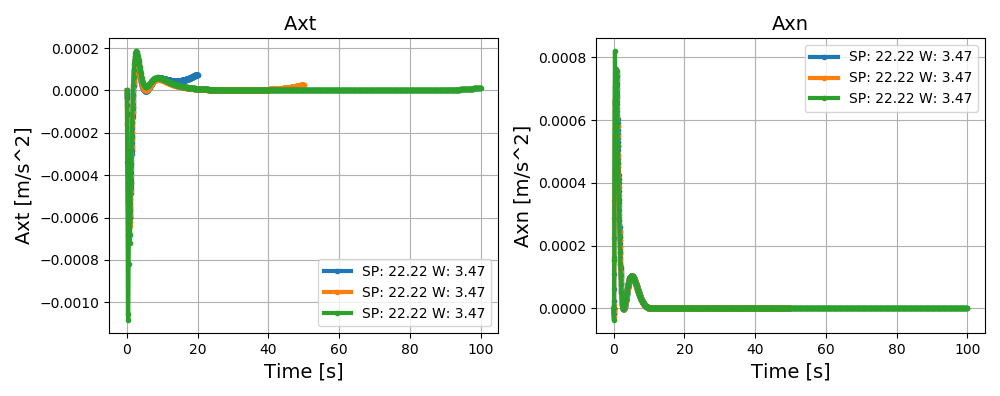
\includegraphics[width=1.0\textwidth]{10t.png}
	\label{fig:lat_acc_val}
\end{figure}


\begin{figure}[h!]
	\centering
	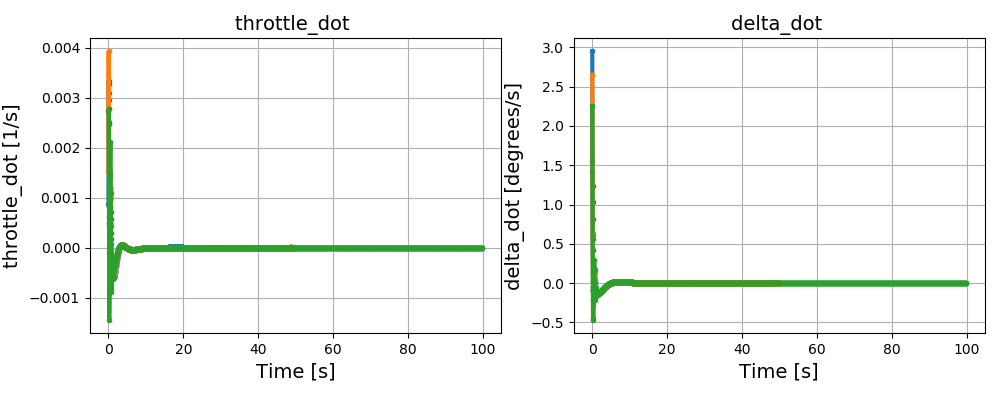
\includegraphics[width=1.0\textwidth]{11t.png}
	\label{fig:lat_acc_val}
\end{figure}


\clearpage

\section{Amount of optimization points}

 \begin{figure}[h!]
	\centering
	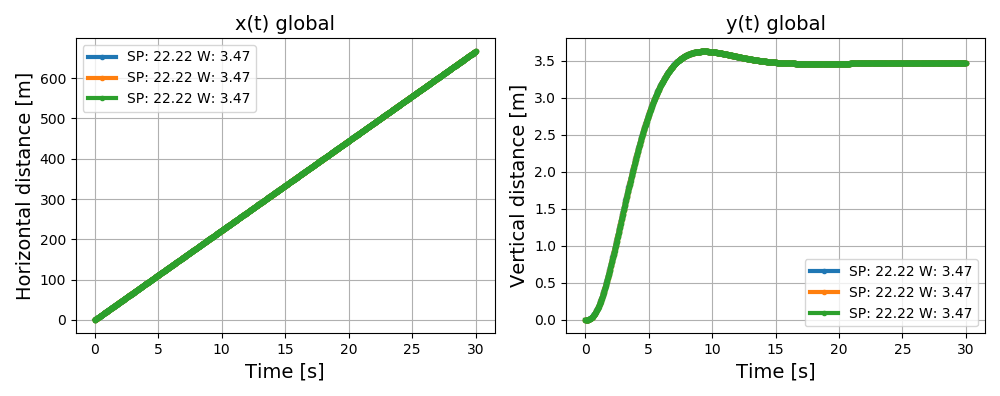
\includegraphics[width=1.0\textwidth]{1.png}
	\label{fig:lat_acc_val}
\end{figure}


\begin{figure}[h!]
	\centering
	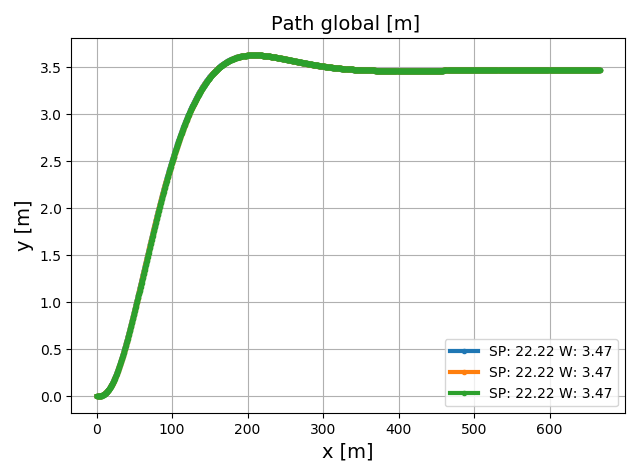
\includegraphics[width=0.8\textwidth]{2.png}
	\label{fig:lat_acc_val}
\end{figure}

\begin{figure}[h!]
	\centering
	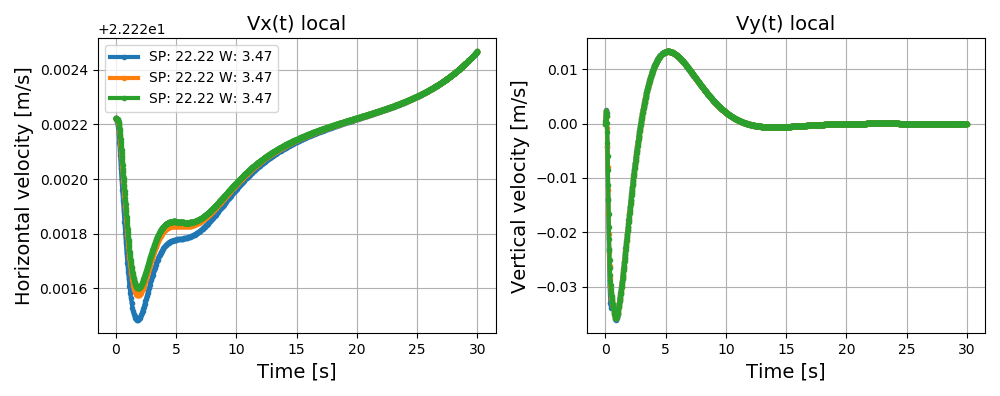
\includegraphics[width=1.0\textwidth]{3.png}
	\label{fig:lat_acc_val}
\end{figure}


\begin{figure}[h!]
	\centering
	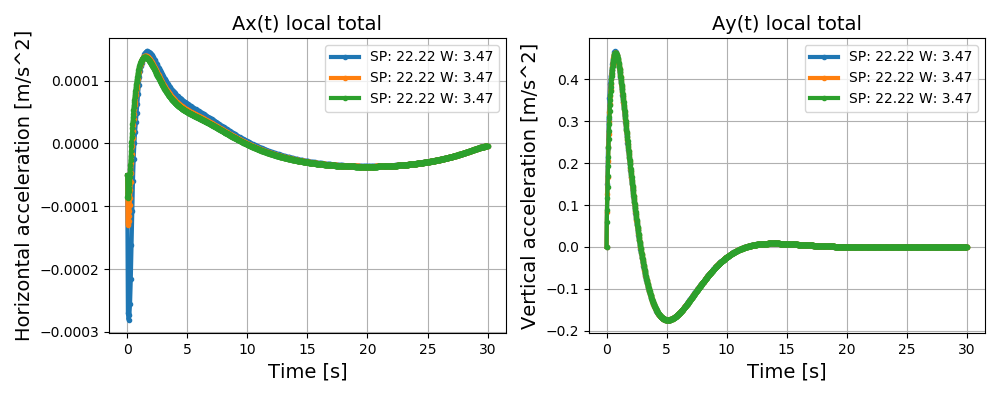
\includegraphics[width=1.0\textwidth]{4.png}
	\label{fig:lat_acc_val}
\end{figure}


\begin{figure}[h!]
	\centering
	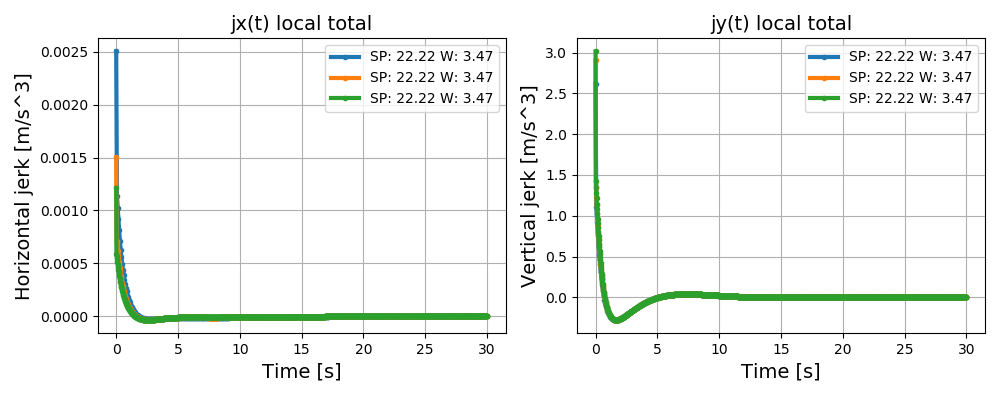
\includegraphics[width=1.0\textwidth]{5.png}
	\label{fig:lat_acc_val}
\end{figure}


\begin{figure}[h!]
	\centering
	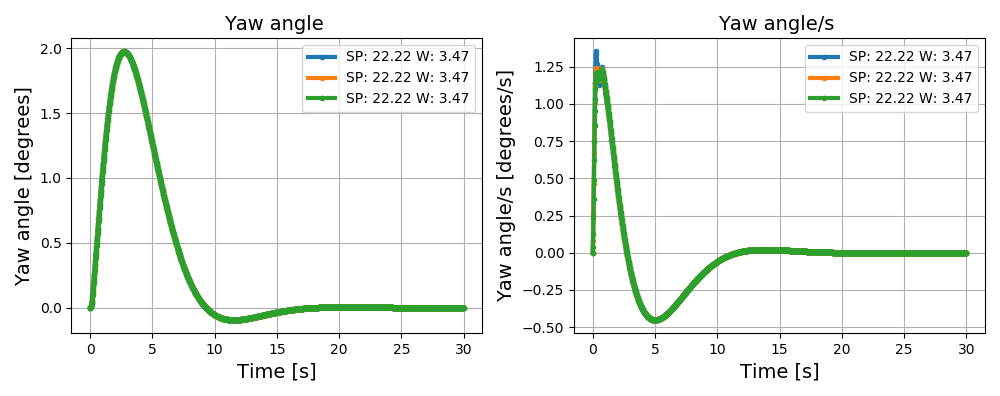
\includegraphics[width=1.0\textwidth]{6.png}
	\label{fig:lat_acc_val}
\end{figure}


\begin{figure}[h!]
	\centering
	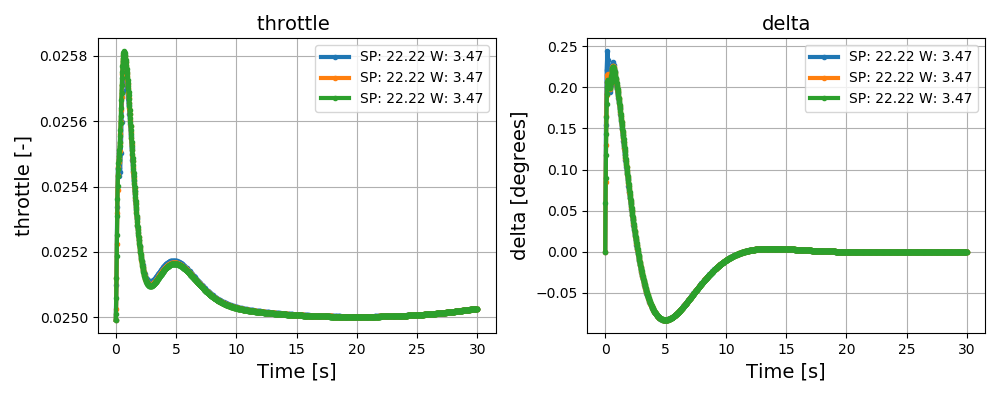
\includegraphics[width=1.0\textwidth]{7.png}
	\label{fig:lat_acc_val}
\end{figure}


\begin{figure}[h!]
	\centering
	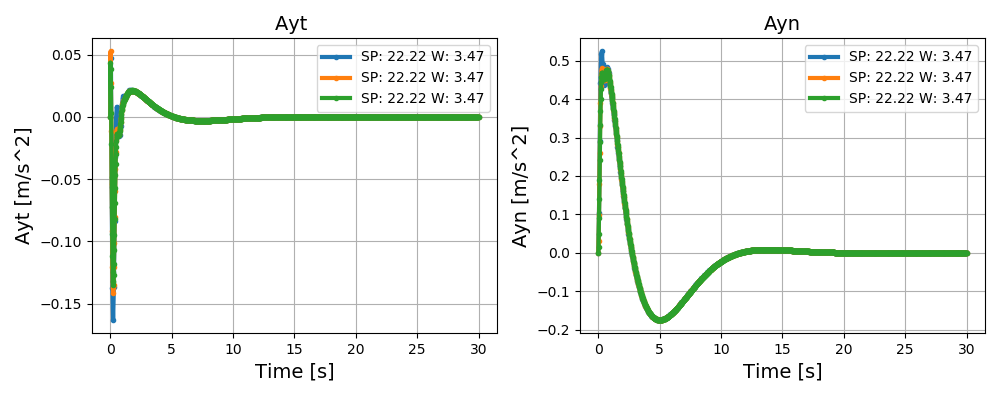
\includegraphics[width=1.0\textwidth]{8.png}
	\label{fig:lat_acc_val}
\end{figure}


\begin{figure}[h!]
	\centering
	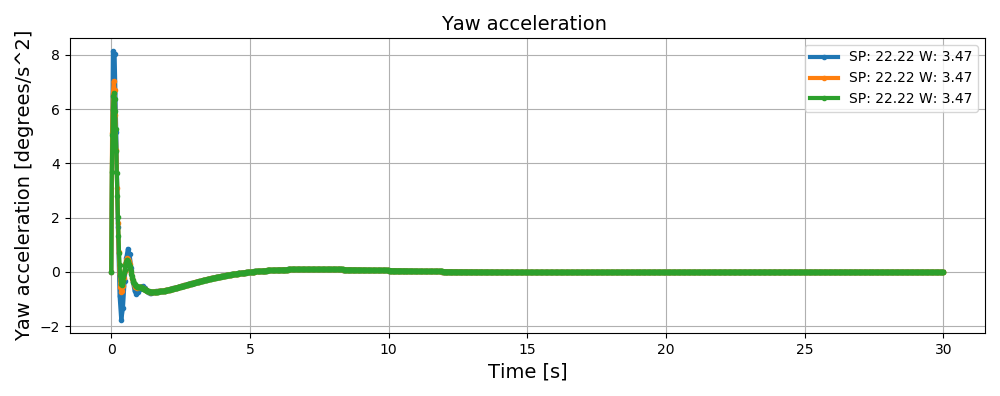
\includegraphics[width=1.0\textwidth]{9.png}
	\label{fig:lat_acc_val}
\end{figure}


\begin{figure}[h!]
	\centering
	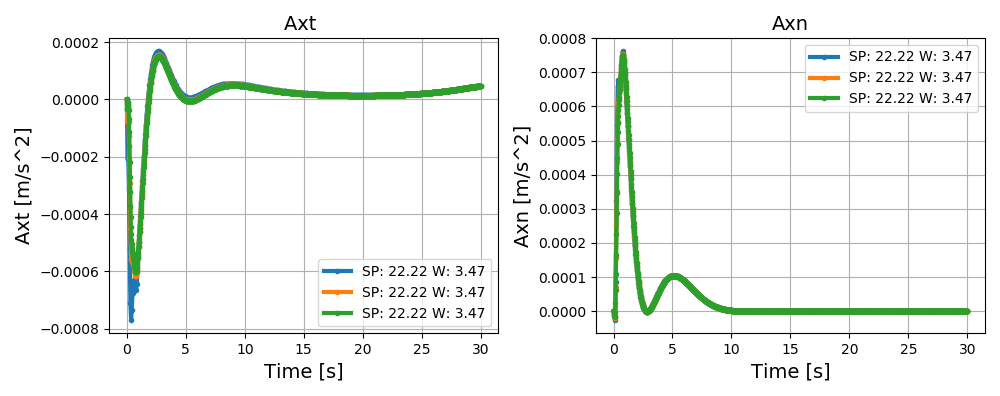
\includegraphics[width=1.0\textwidth]{10.png}
	\label{fig:lat_acc_val}
\end{figure}


\begin{figure}[h!]
	\centering
	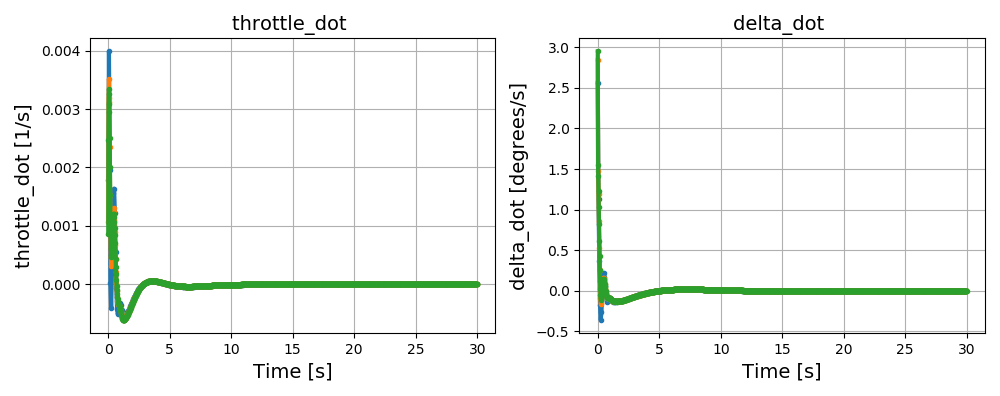
\includegraphics[width=1.0\textwidth]{11.png}
	\label{fig:lat_acc_val}
\end{figure}










%%% Local Variables: 
%%% mode: latex
%%% TeX-master: "thesis"
%%% End: 
